\documentclass[10pt,a4paper]{article}
\usepackage{times}                       % 使用 Times New Roman 字体
\usepackage{CJK,CJKnumb,CJKulem}         % 中文支持宏包
\usepackage{color}                       % 支持彩色

\usepackage{comment}
\usepackage{amsmath}
\usepackage{amssymb}
\usepackage{amsthm}
\usepackage{amscd}
\usepackage{graphicx}
\usepackage{indentfirst}
\usepackage{titlesec}
\usepackage[top=25.4mm, bottom=25.4mm, left=31.7mm, right=32.2mm]{geometry}
\renewcommand{\baselinestretch}{1.5}

%页面设置
\begin{CJK*}{UTF8}{hei}
%\theoremstyle{definition}
%\newtheoremstyle{mythm}{1.5ex plus 1ex minus .2ex}{1.5ex plus 1ex minus .2ex}
%   {\kai}{\parindent}{\song\bfseries}{}{1em}{}
\newtheoremstyle{mythm}{1ex}{1ex}%定理环境的上下间距.
{\CJKfamily{song}}{\parindent}{\CJKfamily{hei} \bf}{}{1em}{}%定理内容为宋体, 缩进, 定理名称为黑粗体
\theoremstyle{mythm}%设置定理环境
\newtheorem{thm}{定理~}[section]
\newtheorem{lem}[thm]{引理~}
\newtheorem{pro}[thm]{性质~}
\newtheorem{fact}[thm]{Fact}
\newtheorem{prop}[thm]{命题~}
\newtheorem{ques}[thm]{问题~}
\newtheorem{cor}[thm]{推论~}
\newtheorem{de}[thm]{定义~}
\newtheorem{rem}[thm]{注记~}
\numberwithin{equation}{section}
\end{CJK*}
\renewcommand\refname{\CJKfamily{hei}参考文献}
%\renewcommand{\abstractname}{摘要}
%%%%%%%%%%%%%%%%下面几行用于改变证明环境的定义
\makeatletter
\renewenvironment{proof}[1][\proofname]{\par
\pushQED{\qed}%
\normalfont \topsep6\p@\@plus6\p@ \labelsep1em\relax
\trivlist
\item[\hskip\labelsep\indent
\bfseries #1]\ignorespaces
}{%
\popQED\endtrivlist\@endpefalse
}
\makeatother
%%%%%%%%%%%%%%(http://latex.yo2.cn)
\renewcommand{\proofname}{\CJKfamily{hei}证明}

\renewcommand{\thefootnote}{\fnsymbol{footnote}}
%\titleformat{\section}{\CJKfamily{hei} }{\arabic{section}{1em}{}
\titleformat{\section}{\large \bf \CJKfamily{hei} }{{\bf \thesection\space}}{0pt}{}

\begin{document}
%\setlength{\baselineskip}{1ex}%设置行距
\setlength{\abovedisplayskip}{1ex} %设置公式上边间距
\setlength{\belowdisplayskip}{1ex} %设置公式下边间距
\begin{CJK*}{UTF8}{song}

\author{翁荻 (11621046)}                                 % 作者
\title{图像空间动态全局照明的近似}              % 题目
\maketitle                                           % 生成标题

\section{引言}
对于大型动态场景而言,实时全局照明仍然是一个未解决的问题,我们只能通过一些近似算法保证足够的帧率。
一种常见的近似是环境光遮蔽(Ambient Occlusion, AO),因为其速度快和实现简单而被经常用于电影和计算机游戏的制作中。
环境光遮蔽计算了环境光对场景中每个点的贡献值。例如在渲染一根空心管时,管内部通常比管外表面更暗,且越深相对而言越受遮挡,也就是会变得越来越暗。

\begin{figure}[htbp]
    \vspace{-1mm}
	\centering
  	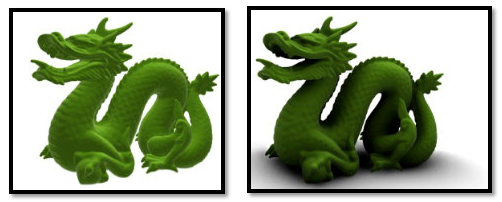
\includegraphics[width=0.75\textwidth]{fig/ao}
    \vspace{-4mm}
  	\caption{环境光遮蔽应用前后对比}
  	\label{fig:ao}
    \vspace{-1mm}
\end{figure}

环境光遮蔽可以看做是为物体表面的每个点都计算了一个对于环境光的接受值。在户外开放的场景中,这个接受值可以用从每个点能看到多少天空来衡量;在室内的场景中,我们通常考虑将墙壁作为环境光的来源,针对每个结点计算某个范围角度的覆盖率。环境光遮蔽经常用作后处理效果,它渲染的结果是漫射,无方向性的阴影效果(图\ref{fig:ao})。环境光遮蔽不会渲染明显的阴影,而是使封闭和遮蔽的区域变暗,并影响渲染图像的整体色调。

典型的环境光遮蔽计算公式如下:
\begin{equation*}
A(p,n)=\frac{1}{\pi}\int_{\Omega}V(\omega,p)\text{max}(\omega\cdot n, 0)d\omega
\end{equation*}
其中的$n$表示几何体元在$p$点外所对应的法向量,$V$为相应的可见函数,$\Omega$表示对应的半球空间,$\omega$表示半球体$\Omega$从$p$点处射出的方向向量。环境光遮蔽值的计算通过对围绕$p$点的半球体上的局部环境光遮蔽值进行积分而得到,由此可见函数$V$为二值函数,即其可能值为$0$或$1$,分别表示在从$p$点处在$n$方向上不可以或可以看到环境中的其它几何体。

环境光遮蔽是一种简单的实时计算环境光的技术。近来,实时计算机图形学社区开始尝试通过复杂的环境光映射来获得具有真实感的光照,而不再是传统的少数几个简单光源。在真实世界里,光实际上是从不同的角度照射到表面上的,而不仅仅是几个点光源或方向光源,这种假设会显著影响视觉效果。人们开发了很多技术来捕捉真实世界中的光照(比如电影中),使得渲染出的光照看起来像是出自于真实环境一样,这样相似性使得图形学可以和真实的场景无缝集成。对于完全合成的场景,可利用场景的环境映射来给场景内的角色或对象增加光照,从而改善渲染结果的真实感。它们不光是用映射处理镜面反射,还用于计算光滑和漫反射表面的光照。

\begin{figure}[htbp]
    \vspace{-1mm}
	\centering
  	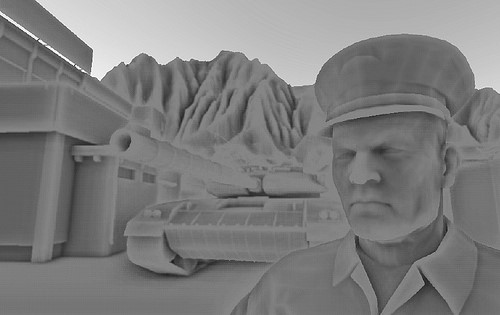
\includegraphics[width=0.75\textwidth]{fig/crytek}
    \vspace{-4mm}
  	\caption{孤岛危机中SSAO效果}
  	\label{fig:crytek}
    \vspace{-1mm}
\end{figure}

在诸如游戏等实时应用的场合中,屏幕空间环境光遮蔽(Screen Space Ambient Occlusion,SSAO)和水平基准环境光遮蔽(Horizon-Based Ambient Occlusion,HBAO)是两类最常见的对真环境光遮蔽的快速近似。它们借助了像素缓冲而非场景几何来计算环境光映射。屏幕空间环境光遮蔽(SSAO)算法最初由 Crytek 公司开发,并随着游戏《孤岛危机》的成功而大受欢迎(图\ref{fig:crytek})。这一技术使用了屏幕空间场景的深度而不是真实的几何体数据来确定遮蔽量。这一做法相对于真正的环境光遮蔽不但速度快,而且还能获得很好的效果,使得它成为近似实时环境光遮蔽的标准。环境光遮挡十分耗费计算资源,Crytek公司想出了一个折中的办法,为每个像素计算一次遮挡因子。这个算法名中的前缀“屏幕空间”,这意味着会依次遍历屏幕空间中的每一个像素,并提取每个像素在视图空间下的坐标信息,并在这个坐标点周围随机采样一些点,判断这些随机点位于几何体内部还是外部。如果许多点都是位于几何体内部,这就表示原始像素应该是位于角落中的因而接收到的光照也较少;如果大部分点都位于几何体之外,这就表示原始像素被“高度曝光”,因此接收到的光照也较多。

然而,现有的环境光遮蔽技术解耦了可见性和照明,只对实际照明情况做出粗略的估计。环境光遮蔽使得凹角变暗,但通常忽略了入射光的所有方向信息。Ritschel等人\cite{Ritschel:2009:SSDO}基于屏幕空间环境光遮蔽发展出一种新型技术,屏幕空间方向遮蔽(Screen-space Directional Occlusion, SSDO),以产生更加贴近真实的光照模型。

%\clearpage % 换页,\newpage也可以,推荐\clearpage

\section{方法概述}

为了计算图像空间中的光线传播,屏幕空间方向遮蔽算法接受一个填满位置和法向量的帧缓冲作为输入\cite{SegoviaIMP06},并经过两轮渲染,一轮计算直射光照和一轮计算间接弹射光照,最后输出一个完成光照计算的像素缓冲。

\subsection{直射光照}

标准屏幕空间环境光遮蔽算法通过计算周围像素对当前像素的平均可见度来点亮一个像素。这个遮挡程度会乘上所有入射方向无遮挡的光照。Ritschel等人提出如下方法以移除遮挡和光照之间的解耦:

对于每个在三维空间中点$P$并且法向量为$n$的像素,直接辐射度$L_{\text{dir}}$可由$N$个均匀分布在半球上的采样方向$\omega_i$计算得到,且每个采样方向覆盖角度为$\Delta\omega=2\pi/N$:
\begin{equation*}
L_{\text{dir}}=\sum^N_{i=1}\frac{\rho}{\pi}L_{\text{in}}(\omega_i)V(\omega_i)\text{cos}\theta_i\Delta\omega
\end{equation*}
每个采样计算了入射辐射度的乘积$L_\text{in}$,可见性$V$和漫反射双向反射分布函数$\rho/\pi$。我们假设$L_\text{in}$可以从点光源或者环境图中高效地计算。为了避免使用光线追踪计算可见性$V$,我们在\textbf{屏幕空间}中做遮挡物的近似。
对于每个采样,我们从点$P$向着方向$\omega_i$前进随机长度$\lambda_i\in\lbrack 0...r_{\text{max}}\rbrack$,其中$r_{\text{max}}$是用户自定义的半径。这样我们可以得到一系列在半球上、以$P$为中心且朝向在$n$周围的采样点集合$P+\lambda_i\omega_i$。
因为我们在$P$点周围的局部帧生成了一系列三维采样点,所以有些采样点会高于表面,而另外一些点会低于表面。在近似的可见性测试中,所有低于几何体表面的采样点被当做遮挡物。图\ref{fig:occluder}左侧展示了一个$N=4$、采样点为$A,B,C,D$的例子:点$A,B,D$低于表面,因此它们被归类为相对于点$P$的遮挡物;而点$C$高于表面,被归类为可见的。

\begin{figure}[htbp]
    \vspace{-1mm}
	\centering
  	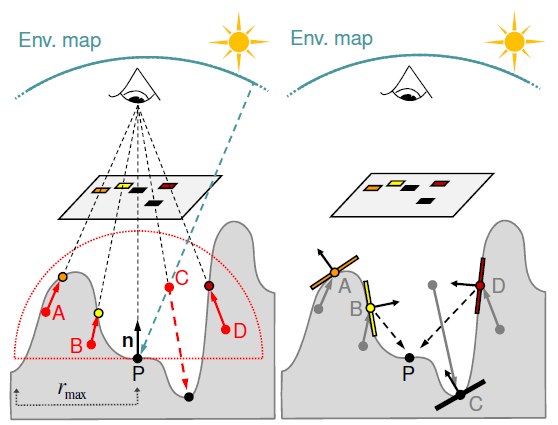
\includegraphics[width=0.75\textwidth]{fig/occluder}
    \vspace{-4mm}
  	\caption{近似的可见性测试}
  	\label{fig:occluder}
    \vspace{-1mm}
\end{figure}

为了测试一个采样点是否可见,采样点被投影到图像。现在,三维位置可以从位置缓冲中读取,而这些点会被投影到物体平面上(红色箭头)。如果一个采样点离观察者的位置因为这个投影缩短了,那这个采样点将被归类为低于表面的。在图\ref{fig:occluder}的例子中,采样点$A,B,D$因为向观察者移动了而被归类为低于表面的,采样点$C$则是向远离观察者方向移动。与屏幕空间环境光遮蔽对比,这个算法不会计算从所有采样点来的光线,而单单只计算从可见方向来的光照(采样点$C$)。包含这一方向信息可以极大提高渲染结果的质量,特别是入射光照在不同方向上有不同的颜色。

\subsection{间接弹射}

为了包含一次光线的间接弹射,我们可以利用上次渲染储存在帧缓冲中的直射光信息:对于每一个被当做遮挡物的采样点($A,B,D$),对应像素的颜色$L_{\text{pixel}}$被用于在表面上的小面片辐射源(图\ref{fig:occluder}右侧所示)。我们在这里考虑源的法向量,防止逆向片源产生的颜色溢出(color bleeding)。周围几何体产生的附加辐射度可以被近似为:
\begin{equation*}
L_{\text{ind}}(P)=\sum^N_{i=1}\frac{\rho}{\pi}L_{\text{pixel}}(1-V(\omega_i))\frac{A_s\text{cos}\theta_{s_i}\text{cos}\theta_{r_i}}{d^2_i}
\end{equation*}
其中,$d_i$是点$P$到遮挡物$i$的距离($d_i$被限定在1以内以避免奇异性问题),$\theta_{s_i}$和$\theta_{r_i}$是源、目标的法向量和发射方向的夹角。$A_s$是小面片的面积。作为面片面积的初始值,我们假定半球上是平的。因此,底圆可以被细分成$N$个区域,每个区域覆盖了面积$A_s=\pi r^2_{\text{max}}/N$。实际的值可能更高,取决于半球中斜率的分布,所以我们可以用这个参数来手动控制颜色溢出。在图\ref{fig:occluder}的例子中,面片$A$没有间接光贡献,因为它的朝向是反的。面片$C$在点$P$的负半空间中,因此也没有贡献。面片$B$和$D$是点$P$的间接光源。

\section{实验结果}

\begin{figure}[htbp]
    \vspace{-3mm}
	\centering
  	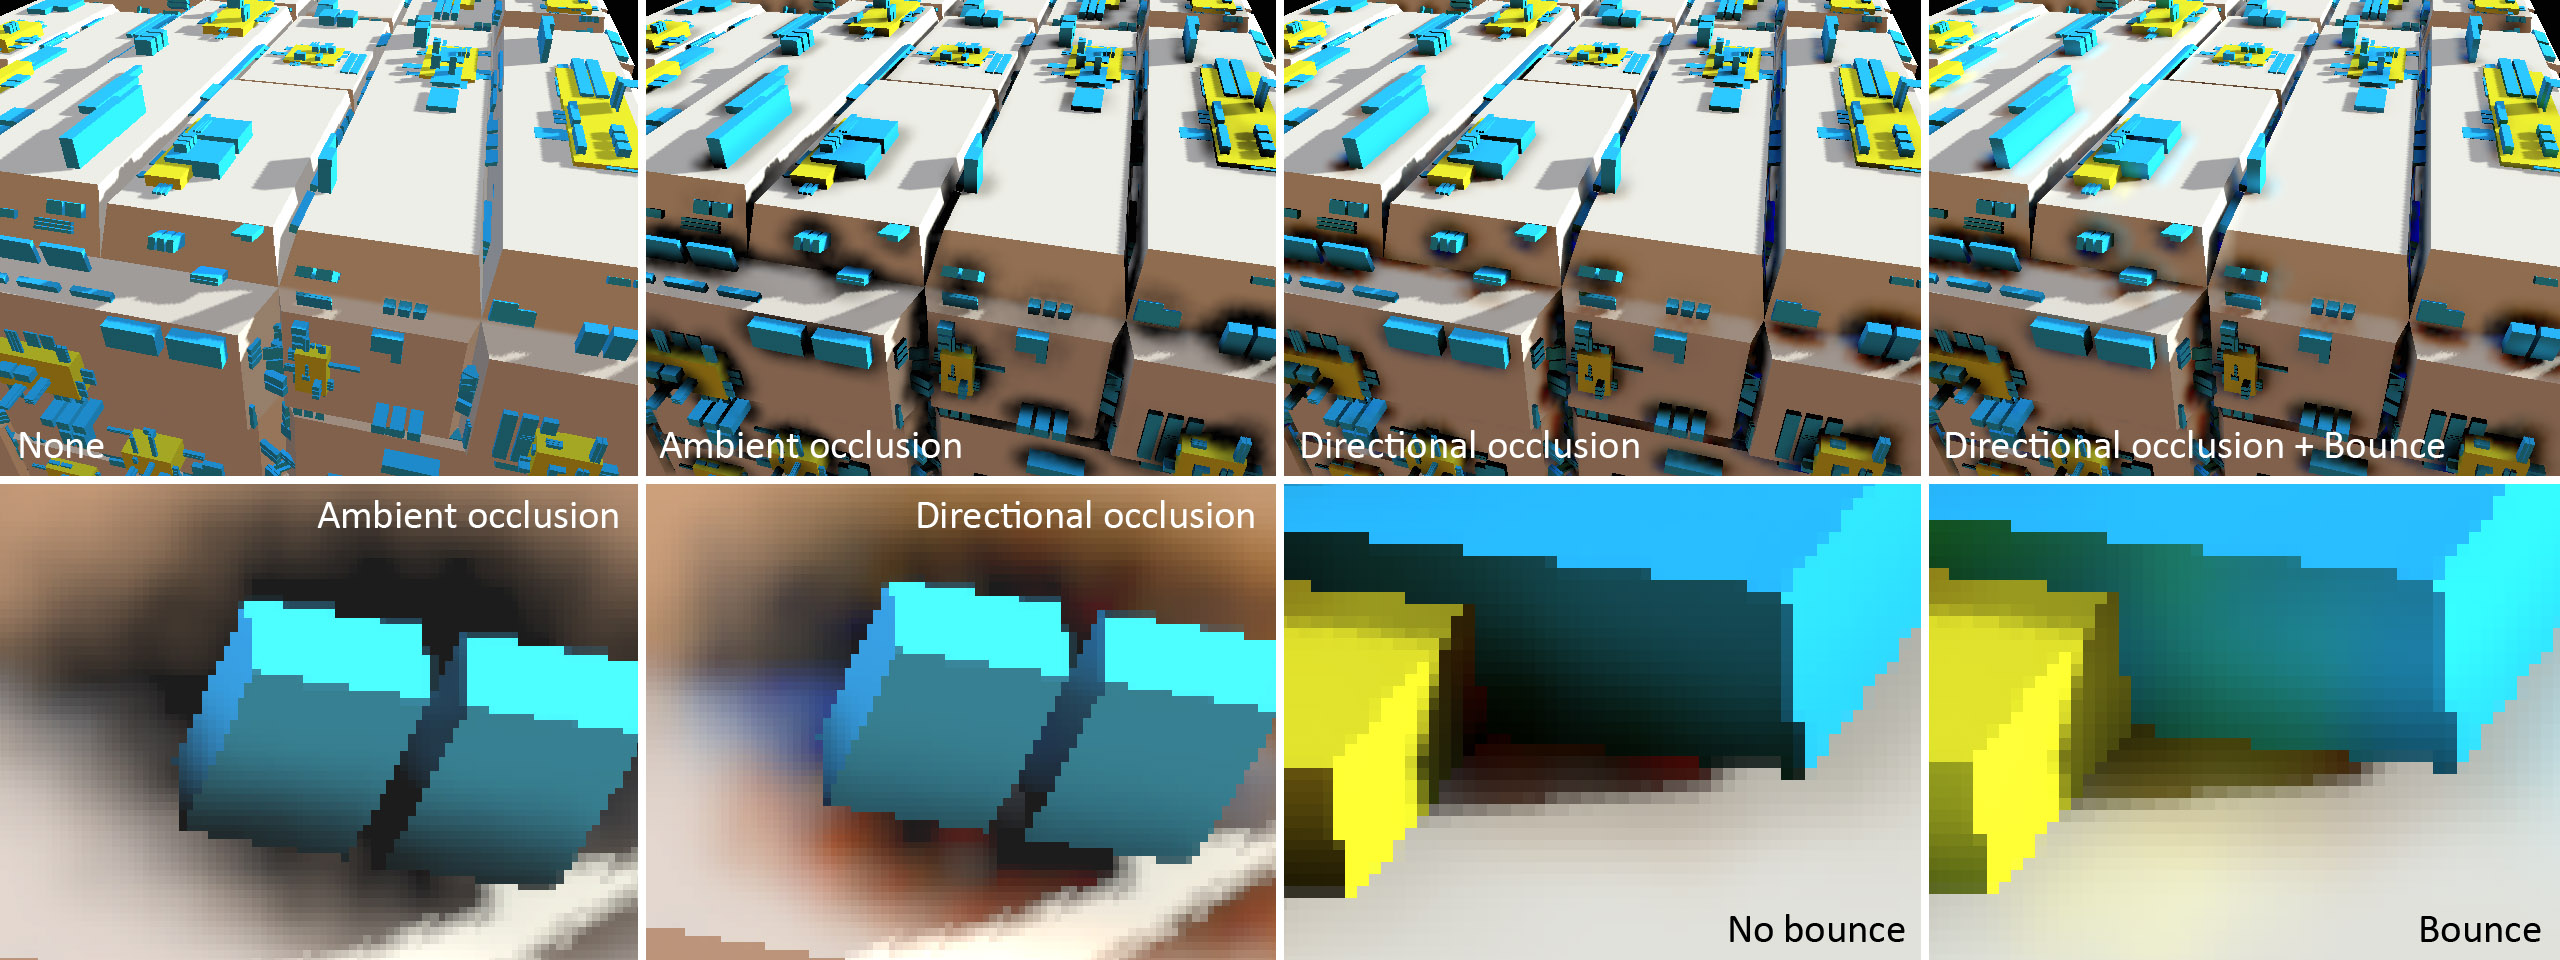
\includegraphics[width=0.9\textwidth]{fig/result}
    \vspace{-4mm}
  	\caption{屏幕空间方向遮蔽的渲染结果与对比}
  	\label{fig:result}
    \vspace{-1mm}
\end{figure}

经典SSAO算法\cite{DBLP:conf/si3d/2007}有着和SSDO算法相似的步骤和计算代价。SSDO需要更多的计算量来评估着色模型,但是在可见性判断上是和SSAO较为相似的。SSDO算法的渲染结果如图\ref{fig:result}所示。SSDO算法可以正确的显示带有颜色的阴影,而SSAO算法仅仅只在每个地点显示灰色阴影。间接弹射的光照效果也同样可从图中观察得到。

\section{小结与讨论}

间接弹射和方向遮挡的引入提高了人对复杂结构的感知,使几何与材质光照变得一致。经典环境光遮蔽的一个问题是光照强度被完全忽略:遮挡物周围的所有东西都同等地变暗,即使光照是各向异性的。
在许多场景中,例如户外天空光源的场景,光照是柔和的,但仍然有强烈的方向性。在变化的光照下使用传统的环境光遮蔽算法会因为阴影保持不变的同时底下着色发生变化而产生主观上的瑕疵。这将会给人一种泥土的错觉,因为反射性的改变(尘埃、泥土、铜绿)是感官上对于这种在不同光照下均匀变暗一种最合理的解释。
利用合适的方向遮挡,复杂结构中的细节将会相对于大尺度上的光照产生合理的阴影(软度、尺寸、方向、颜色等)。

\bibliographystyle{abbrv}
\bibliography{template}
% \begin{thebibliography}{MM}
% \addtolength{\itemsep}{-0.5em}
% \begin{small}
% \bibitem{no} text
% \end{small}
% \end{thebibliography}
% \newpage
\end{CJK*}
\end{document}

